\documentclass[aspectratio=169, 10pt]{beamer}

% -----------------------------------------------------------------------------
% Packages
% -----------------------------------------------------------------------------
\usepackage[utf8]{inputenc}
\usepackage[T1]{fontenc}
\usepackage{lmodern}
\usepackage{amsmath,amssymb}
\usepackage{booktabs}
\usepackage{colortbl}
\usepackage{tabularx}
\usepackage{tcolorbox}
\usepackage{tikz}
\usepackage{hyperref}
\usepackage{microtype}

\usetikzlibrary{arrows.meta, positioning, shapes.geometric, backgrounds, fit, calc, shadows}
\tcbuselibrary{skins}

% -----------------------------------------------------------------------------
% Presentation Metadata
% -----------------------------------------------------------------------------
\title[AI-Powered SOC Assistant \quad\textbar\quad PPD-II Second Review]{AI-Powered Security Operations Center (SOC) Assistant Using Large Language Models}
\subtitle{System Architecture, Evidence-Grounded RAG Pipeline, and Implementation Progress}
\author[Kunal Sanga (2301341031)]{%
  \textbf{Kunal Sanga}\\[2pt]
  {\footnotesize Reg. No.: 2301341031 \quad\textbar\quad Branch: Computer Science and Engineering}\\[4pt]
  {\footnotesize \textbf{Supervised by:} Miss Alka Dash (Assistant Professor, Department of CSE)}
}
\institute[Silicon Institute of Technology, Sambalpur]{%
  Department of Computer Science and Engineering\\
  Silicon Institute of Technology, Sambalpur, Odisha\\[3pt]
  \textbf{PPD-II Second Review \quad\textbar\quad Academic Session 2026--2027}
}
\date{\today}

% -----------------------------------------------------------------------------
% Cybersecurity Theme Colors
% -----------------------------------------------------------------------------
\definecolor{socnavy}{RGB}{11, 25, 44}       % Deep midnight navy
\definecolor{socblue}{RGB}{24, 76, 120}      % Sapphire blue
\definecolor{soccyan}{RGB}{0, 150, 185}      % Cyber cyan accent
\definecolor{soclight}{RGB}{246, 249, 252}   % Soft slide card background
\definecolor{socdarktext}{RGB}{18, 28, 42}   % Primary text
\definecolor{socmuted}{RGB}{90, 105, 125}    % Muted secondary text
\definecolor{socgreen}{RGB}{34, 139, 74}     % Verified / Passing
\definecolor{socamber}{RGB}{210, 105, 30}    % In-progress / Warning
\definecolor{bordergray}{RGB}{215, 225, 238} % Subtle box borders

% -----------------------------------------------------------------------------
% Beamer Layout Customization
% -----------------------------------------------------------------------------
\usecolortheme[named=socblue]{structure}
\setbeamertemplate{navigation symbols}{}
\setbeamertemplate{headline}{}

% Background and fonts
\setbeamercolor{background canvas}{bg=white}
\setbeamercolor{normal text}{fg=socdarktext}
\setbeamercolor{title}{fg=socnavy}
\setbeamercolor{frametitle}{fg=socnavy,bg=soclight}
\setbeamerfont{frametitle}{series=\bfseries,size=\large}
\setbeamerfont{framesubtitle}{size=\footnotesize,series=\normalfont}

% Slide Frame Title Banner
\setbeamertemplate{frametitle}{%
  \begin{tcolorbox}[
    colback=soclight,
    colframe=bordergray,
    boxrule=0.5pt,
    arc=0mm,
    left=6pt,right=6pt,top=4pt,bottom=4pt,
    width=\paperwidth,
    enlarge left by=-1cm,
    enlarge right by=-1cm
  ]
    \parbox[c]{0.78\linewidth}{%
      \usebeamerfont{frametitle}\insertframetitle\par%
      \ifx\insertframesubtitle\@empty\else%
        \vskip1pt{\usebeamerfont{framesubtitle}\textcolor{socmuted}{\insertframesubtitle}}\fi%
    }%
    \hfill%
    \parbox[c]{0.18\linewidth}{\raggedleft%
      
\includegraphics[height=0.60cm]{sitlogo.png}%
    }
  \end{tcolorbox}%
  \vskip-6pt%
}

% Clean, Professional Footline
\setbeamertemplate{footline}{%
  \begin{tcolorbox}[
    colback=socnavy,
    colframe=socnavy,
    arc=0mm,
    boxrule=0pt,
    left=8pt,right=8pt,top=2.5pt,bottom=2.5pt,
    width=\paperwidth,
    enlarge left by=-1cm,
    enlarge right by=-1cm
  ]
    \textcolor{white}{\footnotesize\insertshortauthor}
    \hfill
    \textcolor{soccyan!80}{\footnotesize\textbf{\insertshorttitle}}
    \hfill
    \textcolor{white}{\footnotesize\textbf{\insertframenumber{} / \inserttotalframenumber}}
  \end{tcolorbox}%
}

% Itemize customization
\setbeamertemplate{itemize item}{\textcolor{soccyan}{\scriptsize$\blacksquare$}}
\setbeamertemplate{itemize subitem}{\textcolor{socblue}{\tiny$\blacktriangleright$}}
\setlength{\leftmargini}{1.0em}

% Custom Card Boxes
\newtcolorbox{cardbox}[3]{
  colback=#1,
  colframe=#2,
  coltitle=white,
  title={\scriptsize\textbf{#3}},
  arc=1.2mm,
  boxrule=0.7pt,
  left=4pt,right=4pt,top=3pt,bottom=3pt,
  fontupper=\scriptsize
}

% =============================================================================
% PRESENTATION SLIDES
% =============================================================================
\begin{document}

% -----------------------------------------------------------------------------
% SLIDE 1: Title Slide
% -----------------------------------------------------------------------------
\begin{frame}[plain]
  \vspace{-0.1cm}
  \begin{tcolorbox}[
    colback=socnavy,
    colframe=socblue,
    boxrule=1.5pt,
    arc=2mm,
    width=\textwidth,
    top=7pt,bottom=7pt,left=12pt,right=12pt
  ]
    \begin{columns}[c]
      \begin{column}{0.80\textwidth}
        \textcolor{soccyan}{\footnotesize\textbf{B.Tech Computer Science \& Engineering \quad\textbar\quad PPD-II Second Review}}\\[3pt]
        {\large\textbf{\textcolor{white}{AI-Powered Security Operations Center (SOC) Assistant}}}\\[2pt]
        {\large\textbf{\textcolor{soccyan!90}{Using Large Language Models}}}\\[3pt]
        {\scriptsize\textcolor{white!80}{Evidence-Grounded RAG, MITRE ATT\&CK / NVD Knowledge Retrieval, and System Implementation}}
      \end{column}
      \begin{column}{0.18\textwidth}
        \raggedleft
        
\includegraphics[width=1.5cm]{sitlogo.png}
      \end{column}
    \end{columns}
  \end{tcolorbox}

  \vspace{0.15cm}

  \begin{columns}[T]
    \begin{column}{0.48\textwidth}
      \begin{tcolorbox}[colback=soclight,colframe=bordergray,arc=1.5mm,boxrule=0.6pt,top=4pt,bottom=4pt,left=6pt,right=6pt]
        {\scriptsize\textbf{\textcolor{socnavy}{Student Investigator:}}}\\[2pt]
        {\small\textbf{Kunal Sanga}} \hfill {\scriptsize Reg. No.: \textbf{2301341031}}\\[1pt]
        {\scriptsize Department of Computer Science \& Engineering}\\[1pt]
        {\scriptsize Silicon Institute of Technology, Sambalpur}
      \end{tcolorbox}
    \end{column}
    \begin{column}{0.48\textwidth}
      \begin{tcolorbox}[colback=soclight,colframe=bordergray,arc=1.5mm,boxrule=0.6pt,top=4pt,bottom=4pt,left=6pt,right=6pt]
        {\scriptsize\textbf{\textcolor{socnavy}{Faculty Project Guide:}}}\\[2pt]
        {\small\textbf{Miss Alka Dash}}\\[1pt]
        {\scriptsize Assistant Professor, Department of CSE}\\[1pt]
        {\scriptsize Silicon Institute of Technology, Sambalpur}
      \end{tcolorbox}
    \end{column}
  \end{columns}

  \vspace{0.15cm}
  \centering
  \textcolor{socmuted}{\scriptsize\textbf{Review Requirements Addressed:} (1) System/Design Development \quad\textbar\quad (2) Implementation Progress \quad\textbar\quad (3) Technical Approach \quad\textbar\quad (4) Preliminary Results}
\end{frame}

% -----------------------------------------------------------------------------
% SLIDE 2: Problem Statement and Research Motivation
% -----------------------------------------------------------------------------
\begin{frame}{Problem Statement \& Objectives}{Operational Challenges in Modern SOCs and Project Scope}
  \begin{columns}[T]
    \begin{column}{0.50\textwidth}
      \begin{cardbox}{soclight}{socblue}{SOC Operational Bottlenecks}
        \begin{itemize}\setlength{\itemsep}{2pt}
          \item \textbf{Alert Fatigue \& Volume}: Tier-1 analysts handle thousands of telemetry events per shift; repetitive triage causes critical alert misses.
          \item \textbf{Manual Threat Attribution}: Manually cross-referencing alerts with MITRE ATT\&CK techniques and CVE records significantly slows MTTD.
          \item \textbf{Naive LLM Hallucinations}: Generic LLMs fabricate non-existent CVEs and cite phantom techniques without verifiable audit trails.
        \end{itemize}
      \end{cardbox}
    \end{column}

    \begin{column}{0.50\textwidth}
      \begin{cardbox}{soclight}{soccyan!90!black}{Project Research Objectives}
        \begin{itemize}\setlength{\itemsep}{2pt}
          \item \textbf{Evidence-Grounded AI Assistant}: Develop an advisory pipeline citing verified security knowledge (1,762 indexed chunks).
          \item \textbf{Data Privacy \& Zero Cloud Leakage}: Run entirely on-premise using local Ollama (\texttt{qwen3:8b}) and Qdrant.
          \item \textbf{Verifiable Decision Provenance}: Enforce citation validation where every claim references retrieved evidence IDs.
          \item \textbf{Human-in-the-Loop}: Deliver advisory recommendations; no unvalidated automated remediation.
        \end{itemize}
      \end{cardbox}
    \end{column}
  \end{columns}

  \vspace{0.15cm}
  \begin{tcolorbox}[colback=socnavy!5,colframe=socblue,boxrule=0.5pt,arc=1mm,top=3pt,bottom=3pt,left=6pt,right=6pt]
    \scriptsize\textbf{Research Scope Distinction:} Retrieval and LLM enrichment structure evidence for the analyst; they do not replace human analyst verification or claim zero-hallucination guarantees without automated validation.
  \end{tcolorbox}
\end{frame}

% -----------------------------------------------------------------------------
% SLIDE 3: System/Design Development: High-Level Architecture
% -----------------------------------------------------------------------------
\begin{frame}{System/Design Development}{High-Level Multi-Tier System Architecture}
  \centering
  \resizebox{!}{0.64\textheight}{%
  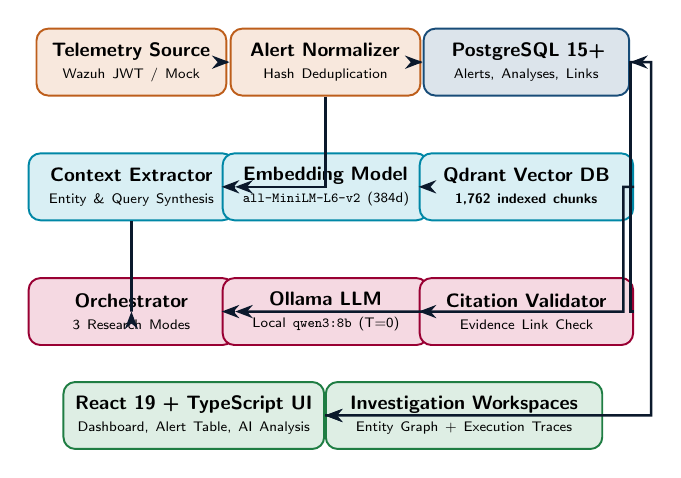
\begin{tikzpicture}[
    scale=0.88,
    font=\sffamily\scriptsize,
    box/.style={rectangle, draw=socnavy, fill=soclight, rounded corners=1.5mm, text centered, inner sep=3pt, line width=0.7pt, minimum height=0.85cm},
    ingest/.style={box, fill=socamber!15, draw=socamber!90!black},
    db/.style={box, fill=socblue!15, draw=socblue},
    rag/.style={box, fill=soccyan!15, draw=soccyan!90!black},
    llm/.style={box, fill=purple!15, draw=purple!80!black},
    ui/.style={box, fill=socgreen!15, draw=socgreen!90!black},
    arrow/.style={-{Stealth[scale=0.9]}, line width=0.9pt, color=socnavy}
  ]
    % Tier 1: Ingestion
    \node[ingest, text width=2.2cm] (wazuh) at (0,3.6) {\textbf{Telemetry Source}\\ \tiny Wazuh JWT / Mock};
    \node[ingest, text width=2.2cm] (norm) at (2.8,3.6) {\textbf{Alert Normalizer}\\ \tiny Hash Deduplication};

    % Tier 2: Storage
    \node[db, text width=2.4cm] (pg) at (5.7,3.6) {\textbf{PostgreSQL 15+}\\ \tiny Alerts, Analyses, Links};

    % Tier 3: RAG & Knowledge
    \node[rag, text width=2.4cm] (ctx) at (0,1.8) {\textbf{Context Extractor}\\ \tiny Entity \& Query Synthesis};
    \node[rag, text width=2.4cm] (embed) at (2.8,1.8) {\textbf{Embedding Model}\\ \tiny \texttt{all-MiniLM-L6-v2} (384d)};
    \node[rag, text width=2.5cm] (qdrant) at (5.7,1.8) {\textbf{Qdrant Vector DB}\\ \tiny \textbf{1,762 indexed chunks}};

    % Tier 4: LLM Orchestrator
    \node[llm, text width=2.4cm] (orch) at (0,0.0) {\textbf{Orchestrator}\\ \tiny 3 Research Modes};
    \node[llm, text width=2.4cm] (ollama) at (2.8,0.0) {\textbf{Ollama LLM}\\ \tiny Local \texttt{qwen3:8b} (T=0)};
    \node[llm, text width=2.5cm] (val) at (5.7,0.0) {\textbf{Citation Validator}\\ \tiny Evidence Link Check};

    % Tier 5: Frontend UI
    \node[ui, text width=3.1cm] (react) at (0.9,-1.5) {\textbf{React 19 + TypeScript UI}\\ \tiny Dashboard, Alert Table, AI Analysis};
    \node[ui, text width=3.3cm] (graph) at (4.8,-1.5) {\textbf{Investigation Workspaces}\\ \tiny Entity Graph + Execution Traces};

    % Connectors
    \draw[arrow] (wazuh) -- (norm);
    \draw[arrow] (norm) -- (pg);
    \draw[arrow] (norm) |- (ctx);
    \draw[arrow] (ctx) -- (embed);
    \draw[arrow] (embed) -- (qdrant);
    \draw[arrow] (ctx) |- (orch);
    \draw[arrow] (qdrant) -- ++(1.4,0) |- (orch);
    \draw[arrow] (orch) -- (ollama);
    \draw[arrow] (ollama) -- (val);
    \draw[arrow] (val) -- ++(1.5,0) |- (pg);
    \draw[arrow] (pg) -- ++(1.8,0) |- (react);
    \draw[arrow] (react) -- (graph);
  \end{tikzpicture}%
  }
  \vspace{0.05cm}
  \begin{columns}[T]
    \begin{column}{0.33\textwidth}
      \scriptsize\textbf{\textcolor{socamber!90!black}{[1] Ingestion:}} Wazuh client / labeled dev mock; hash deduplication in DB.
    \end{column}
    \begin{column}{0.33\textwidth}
      \scriptsize\textbf{\textcolor{soccyan!90!black}{[2] RAG Tier:}} Qdrant indexed with 1,618 MITRE techniques and 144 CVEs.
    \end{column}
    \begin{column}{0.33\textwidth}
      \scriptsize\textbf{\textcolor{purple!80!black}{[3] Reasoning:}} Local Qwen3-8B with strict citation validation before storage.
    \end{column}
  \end{columns}
\end{frame}

% -----------------------------------------------------------------------------
% SLIDE 4: System/Design Development: Workflow & Data Flow
% -----------------------------------------------------------------------------
\begin{frame}{System/Design Development}{Verified Workflow \& End-to-End Processing Path}
  \begin{columns}[T]
    \begin{column}{0.62\textwidth}
      \begin{enumerate}\setlength{\itemsep}{3pt}\scriptsize
        \item \textbf{Alert Ingestion \& Normalization}: Ingests raw Wazuh telemetry; parses timestamp, agent, rule ID, description, source/destination IPs into unified schema.
        \item \textbf{Context Extraction \& Query Synthesis}: Extracts IoCs and generates targeted queries: (a) rule-centric query, (b) MITRE technique anchor, (c) entity context.
        \item \textbf{Dense Semantic Retrieval (Qdrant)}: Computes 384-d cosine similarity over 1,762 knowledge chunks; returns top-$k$ evidence items.
        \item \textbf{Evidence-Constrained Prompting}: Injects structured evidence cards into system prompt with explicit instructions prohibiting uncited claims.
        \item \textbf{Local LLM Inference}: Local Ollama runs \texttt{qwen3:8b} at temperature 0.0 for deterministic, private reasoning.
        \item \textbf{Evidence-Reference Validation}: Automated validator verifies model citations match retrieved evidence IDs before PostgreSQL persistence.
      \end{enumerate}
    \end{column}

    \begin{column}{0.38\textwidth}
      \begin{cardbox}{soclight}{socblue}{Pipeline Trace Verification}
        \scriptsize
        \textbf{Execution Stages Instrumented:}
        \begin{itemize}\setlength{\itemsep}{1.5pt}
          \item Ingestion $\to$ 1--5 ms
          \item Normalization $\to$ 2--8 ms
          \item Embedding generation $\to$ 30--60 ms
          \item Qdrant Vector search $\to$ 8--25 ms
          \item LLM Inference (\texttt{qwen3:8b}) $\to$ 35--80 s
          \item Citation Validation $\to$ 1--3 ms
        \end{itemize}
        \vspace{2pt}
        \textcolor{socnavy}{\textbf{Integrity Check:}} Persisted analyses store evidence foreign-key IDs linking exact retrieved chunks.
      \end{cardbox}
    \end{column}
  \end{columns}
\end{frame}

% -----------------------------------------------------------------------------
% SLIDE 5: Technical Approach: Technology Stack & Core Decisions
% -----------------------------------------------------------------------------
\begin{frame}{Technical Approach}{Technology Stack Rationale \& Architectural Decisions}
  \centering
  \resizebox{0.93\textwidth}{!}{%
  \begin{tabular}{l p{3.6cm} p{9.2cm} c}
    \toprule
    \textbf{Component} & \textbf{Technology Selected} & \textbf{Engineering \& Research Rationale} & \textbf{Status} \\
    \midrule
    \textbf{Backend API} & FastAPI (Python 3.11/13) & High-performance async REST API with typed Pydantic V2 schemas & \textcolor{socgreen}{\textbf{Verified}} \\
    \textbf{Relational DB} & PostgreSQL 15+ / Alembic & ACID transactions for alert logs, analyses, and evidence foreign-key links & \textcolor{socgreen}{\textbf{Verified}} \\
    \textbf{Vector DB} & Qdrant (v1.18+) & Fast cosine HNSW indexing with exact payload filtering ($<$10ms lookup) & \textcolor{socgreen}{\textbf{Verified}} \\
    \textbf{Embeddings} & \texttt{all-MiniLM-L6-v2} & 384-dimensional dense vectors, lightweight local CPU/GPU inference & \textcolor{socgreen}{\textbf{Verified}} \\
    \textbf{Local LLM} & Ollama / \texttt{qwen3:8b} & 8B parameter local reasoning, temp=0.0; guarantees telemetry privacy & \textcolor{socgreen}{\textbf{Verified}} \\
    \textbf{Analyst UI} & React 19 + TypeScript & Modern single-page app, dark SOC theme, interactive canvas, Vite build & \textcolor{socgreen}{\textbf{Verified}} \\
    \textbf{Telemetry} & Wazuh JWT / Mock Client & Real JWT auth protocol implemented; deterministic mock client for tests & \textcolor{socamber}{\textbf{Client Verified}} \\
    \textbf{Containers} & Docker Compose & Single-command orchestration (\texttt{docker compose up}) with healthchecks & \textcolor{socgreen}{\textbf{Verified}} \\
    \bottomrule
  \end{tabular}%
  }

  \vspace{0.08cm}
  \begin{tcolorbox}[colback=socnavy!5,colframe=socblue,boxrule=0.5pt,arc=1mm,top=2.5pt,bottom=2.5pt,left=6pt,right=6pt]
    \scriptsize\textbf{Architectural Key Takeaway:} On-premise execution preserves confidential threat data; hybrid entity-aware retrieval anchors MITRE ATT\&CK techniques and CVE IDs to eliminate hallucinated intelligence.
  \end{tcolorbox}
\end{frame}

% -----------------------------------------------------------------------------
% SLIDE 6: Technical Approach: Evaluation Methodology
% -----------------------------------------------------------------------------
\begin{frame}{Technical Approach: Evaluation Methodology}{Controlled Tri-Mode Experiment Design \& Quantitative Metrics}
  \begin{columns}[T]
    \begin{column}{0.50\textwidth}
      \begin{cardbox}{soclight}{socblue}{Controlled 3-Mode Comparison}
        \begin{itemize}\setlength{\itemsep}{2pt}
          \item \textbf{Mode 1 (\texttt{llm\_only})}: Baseline. Alert passed to Qwen3-8B without external knowledge; measures raw parametric recall.
          \item \textbf{Mode 2 (\texttt{standard\_rag})}: Single unanchored query from rule text; tests basic vector retrieval.
          \item \textbf{Mode 3 (\texttt{evidence\_aware})}: Multi-query synthesis, entity anchoring, hybrid retrieval, and strict citation validation.
        \end{itemize}
      \end{cardbox}

      \begin{cardbox}{soclight}{soccyan!90!black}{Evaluation Datasets}
        \begin{itemize}\setlength{\itemsep}{1.5pt}
          \item \textbf{Dataset v1}: 8 multi-stage scenarios (smoke baseline).
          \item \textbf{Dataset v2}: 40 synthetic scenarios across 7 attack categories + benign controls ($40 \times 3 = 120$ planned evaluations).
        \end{itemize}
      \end{cardbox}
    \end{column}

    \begin{column}{0.50\textwidth}
      \begin{cardbox}{soclight}{socnavy}{Quantitative Metric Suite}
        \begin{itemize}\setlength{\itemsep}{2pt}
          \item \textbf{Technique Detection}: Exact-match Precision, Recall, and F1 score against MITRE ATT\&CK ground truth.
          \item \textbf{Vulnerability Matching}: CVE Precision, Recall, F1 against reference CVE identifiers.
          \item \textbf{Citation Integrity}: Valid evidence reference rate (\% cited IDs present in retrieved evidence set).
          \item \textbf{Retrieval Ranking}: Recall@1, Recall@5, and Mean Reciprocal Rank (MRR) for target knowledge chunks.
          \item \textbf{System Latencies}: Wall-clock end-to-end latency and LLM inference generation latency (seconds).
          \item \textbf{False Alarm Rate}: Severity inflation on benign negative control scenarios.
        \end{itemize}
      \end{cardbox}
    \end{column}
  \end{columns}
\end{frame}

% -----------------------------------------------------------------------------
% SLIDE 7: Implementation Progress: Frontend Analyst Workspace
% -----------------------------------------------------------------------------
\begin{frame}{Implementation Progress: Frontend Analyst Workspace}{Operational User Interface Modules \& Interactive Workspaces}
  \begin{columns}[T]
    \begin{column}{0.48\textwidth}
      \begin{cardbox}{soclight}{socblue}{Implemented UI Modules}
        \begin{itemize}\setlength{\itemsep}{2pt}
          \item \textbf{Security Operations Dashboard}: Live alert metrics, severity distribution (Critical, High, Med, Low), and service status.
          \item \textbf{Alert Management Console}: Full alert table with pagination, severity badges, and source IP/agent filtering.
          \item \textbf{AI Advisory \& Analysis View}: Multi-mode analysis selector, structured threat summary, recommended actions, confidence meter.
          \item \textbf{Threat Intelligence Drawer}: Deep-dive view of cited MITRE techniques and CVE descriptions.
        \end{itemize}
      \end{cardbox}
    \end{column}

    \begin{column}{0.48\textwidth}
      \begin{cardbox}{soclight}{soccyan!90!black}{Advanced Research Features}
        \begin{itemize}\setlength{\itemsep}{2pt}
          \item \textbf{Obsidian-Style Entity Graph}: Force-directed interactive canvas linking alerts, IPs, hosts, usernames, and MITRE techniques (\texttt{EntityGraphPage.tsx}).
          \item \textbf{Execution Trace Waterfall}: Real-time visual timeline showing per-stage latency from ingestion to LLM response (\texttt{ExecutionTracesPage.tsx}).
          \item \textbf{Evaluation Benchmark UI}: Visual progress dashboard displaying real-time metrics across test runs (\texttt{Evaluation.tsx}).
        \end{itemize}
      \end{cardbox}
    \end{column}
  \end{columns}

  \vspace{0.12cm}
  \begin{tcolorbox}[colback=socgreen!10,colframe=socgreen!80!black,boxrule=0.6pt,arc=1mm,top=3pt,bottom=3pt,left=6pt,right=6pt]
    \scriptsize\textbf{UI Honesty \& Validation:} Prominent \texttt{MockDataDisclaimer} warns analysts whenever development/mock telemetry is active. No silent mock fallbacks. \textbf{32 passed frontend unit tests} across 8 test suites.
  \end{tcolorbox}
\end{frame}

% -----------------------------------------------------------------------------
% SLIDE 8: Implementation Progress: Backend Services & Integration
% -----------------------------------------------------------------------------
\begin{frame}{Implementation Progress: Backend Services \& Integration}{Knowledge Base Ingestion, Database Schemas, and API Architecture}
  \begin{columns}[T]
    \begin{column}{0.50\textwidth}
      \begin{cardbox}{soclight}{socblue}{Core Backend Services Verified}
        \begin{itemize}\setlength{\itemsep}{1.5pt}
          \item \textbf{REST API Endpoints}:
            \begin{itemize}\tiny
              \item \texttt{/api/v1/alerts}: Ingestion, filtering, details
              \item \texttt{/api/v1/analysis}: 3-mode analysis execution
              \item \texttt{/api/v1/graph}: Entity relationship graph data
              \item \texttt{/api/v1/evaluation}: Benchmark trigger and reports
              \item \texttt{/api/v1/health}: Readiness probes for DB and Ollama
            \end{itemize}
          \item \textbf{Knowledge Indexing Pipeline}:
            \begin{itemize}\tiny
              \item Automated parsing of MITRE Enterprise ATT\&CK (v14)
              \item Automated parsing of NVD CVE security feed
              \item Total indexed knowledge: \textbf{1,762 vector chunks}
            \end{itemize}
        \end{itemize}
      \end{cardbox}
    \end{column}

    \begin{column}{0.50\textwidth}
      \begin{cardbox}{soclight}{soccyan!90!black}{System Integration Status}
        \begin{itemize}\setlength{\itemsep}{1.5pt}
          \item \textbf{PostgreSQL 15+ Schema}: Structured tables for \texttt{alerts}, \texttt{analyses}, and foreign-key \texttt{evidence} citations.
          \item \textbf{Qdrant Vector Store}: Initialized collection \texttt{security\_knowledge} with 384-d cosine similarity.
          \item \textbf{Wazuh Integration}: Real client with JWT authentication protocol implemented; mock client active for repeatable offline benchmarks.
          \item \textbf{One-Command Dockerization}: \texttt{docker-compose.yml} orchestrates DB, Qdrant, backend, frontend, and auto-seeding.
        \end{itemize}
      \end{cardbox}
    \end{column}
  \end{columns}
\end{frame}

% -----------------------------------------------------------------------------
% SLIDE 9: Implementation Progress: Software Testing & Verification Status
% -----------------------------------------------------------------------------
\begin{frame}{Implementation Progress: Software Testing Status}{Empirical Software Engineering Validation Across Frontend \& Backend}
  \begin{columns}[T]
    \begin{column}{0.48\textwidth}
      \begin{cardbox}{soclight}{socgreen!80!black}{Frontend Test Suite (Vitest v5.0.1)}
        \begin{itemize}\setlength{\itemsep}{1.5pt}
          \item \textbf{Status}: \textcolor{socgreen}{\textbf{100\% Passing}} (8 files, 32 tests)
          \item \textbf{Execution Duration}: 26.43 seconds
          \item \textbf{Test Coverage by Module}:
            \begin{itemize}\tiny
              \item \texttt{App.test.tsx} (Navigation \& routes)
              \item \texttt{Layout.test.tsx} (Header, drawer, theme)
              \item \texttt{Dashboard.test.tsx} (Metric calculations)
              \item \texttt{Alerts.test.tsx} (Filter \& empty states)
              \item \texttt{AIAnalysis.test.tsx} (Mode execution)
              \item \texttt{EntityGraphPage.test.tsx} (Graph render)
              \item \texttt{ExecutionTracesPage.test.tsx} (Traces)
              \item \texttt{Evaluation.test.tsx} (Run tracking)
            \end{itemize}
        \end{itemize}
      \end{cardbox}
    \end{column}

    \begin{column}{0.48\textwidth}
      \begin{cardbox}{soclight}{socblue}{Backend Test Suite (Pytest v9.1.1)}
        \begin{itemize}\setlength{\itemsep}{1.5pt}
          \item \textbf{Status}: \textcolor{socgreen}{\textbf{221 Passed}}, 0 Failed (7 warnings)
          \item \textbf{Execution Duration}: 46.89 seconds (Python 3.13)
          \item \textbf{Verified Subsystems}:
            \begin{itemize}\tiny
              \item Alert normalization \& deduplication
              \item Security context \& IoC extraction
              \item Semantic embeddings (MiniLM-L6-v2)
              \item Qdrant vector store indexing \& search
              \item Ollama provider \& JSON schema parsing
              \item Orchestrator modes \& citation validator
              \item Evaluation metrics \& run resumption
            \end{itemize}
        \end{itemize}
      \end{cardbox}
    \end{column}
  \end{columns}

  \vspace{0.12cm}
  \begin{tcolorbox}[colback=socnavy!5,colframe=socnavy,boxrule=0.5pt,arc=1mm,top=2.5pt,bottom=2.5pt,left=6pt,right=6pt]
    \scriptsize\textbf{Research Integrity Rule:} Software tests (221 backend + 32 frontend) validate code correctness and API contracts; they are distinct from threat-detection accuracy evaluated on benchmark datasets.
  \end{tcolorbox}
\end{frame}

% -----------------------------------------------------------------------------
% SLIDE 10: Preliminary Results: Empirical Benchmark Findings
% -----------------------------------------------------------------------------
\begin{frame}{Preliminary Results}{Empirical Findings from Experimental Evaluation Runs}
  \begin{cardbox}{soclight}{socamber!90!black}{Current Benchmark Execution Status (Dataset v2)}
    \scriptsize\textbf{Scope:} 40 synthetic scenarios $\times$ 3 modes = 120 planned evaluations. Run \texttt{20261024-145621-1345d6} currently has \textbf{12 scenarios completed (36 mode-scenario evaluations completed)}, with 84 evaluations pending execution.
  \end{cardbox}

  \vspace{0.08cm}
  \centering
  \resizebox{\textwidth}{!}{%
  \begin{tabular}{l c c c c c c}
    \toprule
    \textbf{Evaluation Mode} & \textbf{Cases ($N$)} & \textbf{Avg Wall Latency} & \textbf{Technique Prec.} & \textbf{Technique Recall} & \textbf{Technique F1} & \textbf{Valid Citation Rate} \\
    \midrule
    \textbf{LLM-Only (Baseline)} & 12 & 36.8 s & 0.500 & 0.417 & 0.444 & N/A (no citations) \\
    \textbf{Standard RAG} & 12 & 82.2 s & 0.500 & 0.417 & 0.444 & \textbf{1.000 (100\%)} \\
    \textbf{Evidence-Aware RAG} & 12 & 79.6 s & 0.500 & 0.417 & 0.444 & \textbf{1.000 (100\%)} \\
    \bottomrule
  \end{tabular}%
  }

  \vspace{0.10cm}
  \begin{columns}[T]
    \begin{column}{0.50\textwidth}
      \begin{cardbox}{soclight}{socblue}{Dataset v1 Baseline ($N=8$, Completed Run)}
        \begin{itemize}\setlength{\itemsep}{1pt}
          \item \textbf{Retrieval Recall@1}: \textbf{1.000} (Evidence-Aware) vs \textbf{0.250} (Standard RAG) vs 0.000 (LLM-Only).
          \item \textbf{Retrieval MRR}: \textbf{1.000} vs \textbf{0.354} for Standard RAG.
          \item \textbf{Technique F1}: 0.833 across all 8 smoke scenarios.
        \end{itemize}
      \end{cardbox}
    \end{column}

    \begin{column}{0.50\textwidth}
      \begin{cardbox}{soclight}{soccyan!90!black}{Retrieval Ablation (No LLM)}
        \begin{itemize}\setlength{\itemsep}{1pt}
          \item \textbf{Semantic Anchored}: Recall@1 = \textbf{1.000}, MRR = \textbf{1.000} (1563 ms).
          \item \textbf{Semantic Unanchored}: Recall@1 = 0.375, MRR = 0.463 (338 ms).
          \item \textbf{Finding}: Entity anchoring dramatically improves top-1 precision of relevant security techniques.
        \end{itemize}
      \end{cardbox}
    \end{column}
  \end{columns}
\end{frame}

% -----------------------------------------------------------------------------
% SLIDE 11: Technical Limitations & Future Work
% -----------------------------------------------------------------------------
\begin{frame}{Limitations, Challenges \& Future Work}{Transparent Engineering Assessment and Development Roadmap}
  \begin{columns}[T]
    \begin{column}{0.50\textwidth}
      \begin{cardbox}{soclight}{socamber!90!black}{Current Technical Limitations}
        \begin{itemize}\setlength{\itemsep}{2pt}
          \item \textbf{Synthetic Evaluation Scenarios}: Benchmark scenarios are simulated; testing against noisy production enterprise logs remains pending.
          \item \textbf{Simulated Wazuh Cluster}: JWT auth client is verified, but operational evaluation uses local mock telemetry due to lack of a live Wazuh cluster.
          \item \textbf{Inference Latency}: Local \texttt{qwen3:8b} inference takes 35--80s on standard hardware; limits high-volume real-time triage.
          \item \textbf{Exact-Match Evaluation}: Metric scorer matches exact MITRE IDs; related sub-techniques receive zero partial score.
        \end{itemize}
      \end{cardbox}
    \end{column}

    \begin{column}{0.50\textwidth}
      \begin{cardbox}{soclight}{socblue}{Planned Development Roadmap}
        \begin{itemize}\setlength{\itemsep}{2pt}
          \item \textbf{Benchmark Completion}: Complete remaining 84 evaluations on Dataset v2 to establish aggregate statistical significance.
          \item \textbf{Live Wazuh SIEM Sandbox}: Deploy a multi-node live Wazuh cluster with Sysmon telemetry ingestion.
          \item \textbf{Analyst Feedback Loop}: Implement UI endpoints for analyst thumbs up/down feedback and database persistence.
          \item \textbf{Model Quantization \& Distillation}: Evaluate quantized 3B models (e.g., Qwen-2.5-3B-Instruct) to achieve sub-10s inference.
        \end{itemize}
      \end{cardbox}
    \end{column}
  \end{columns}
\end{frame}

% -----------------------------------------------------------------------------
% SLIDE 12: Conclusion & Research Contributions
% -----------------------------------------------------------------------------
\begin{frame}{Conclusion \& Summary of Contributions}{Deliverables Achieved for PPD-II Second Review}
  \begin{columns}[T]
    \begin{column}{0.60\textwidth}
      \begin{cardbox}{soclight}{socblue}{Key Contributions Achieved to Date}
        \begin{itemize}\setlength{\itemsep}{2pt}
          \item \textbf{System/Design Development}: Architected and containerized a multi-tier SOC Assistant integrating PostgreSQL, Qdrant, and local Ollama.
          \item \textbf{Technical Approach}: Implemented an evidence-aware RAG pipeline indexing 1,762 MITRE ATT\&CK and NVD chunks with automated citation validation.
          \item \textbf{Implementation Progress}: Built a complete React 19 UI with Obsidian-style Entity Graph, validated by \textbf{221 backend and 32 frontend unit tests}.
          \item \textbf{Preliminary Results}: Verified 100\% valid citation rate and proven superior top-1 retrieval precision (Recall@1 = 1.0 vs 0.25) through entity anchoring.
        \end{itemize}
      \end{cardbox}
    \end{column}

    \begin{column}{0.40\textwidth}
      \begin{tcolorbox}[colback=socnavy,colframe=socblue,boxrule=1pt,arc=2mm,center,top=8pt,bottom=8pt]
        \centering
        \textcolor{white}{\large\textbf{Thank You!}}\\[6pt]
        \textcolor{soccyan}{\footnotesize\textbf{Questions \& Discussion}}\\[10pt]
        \textcolor{white!80}{\scriptsize Kunal Sanga \quad\textbar\quad Reg. 2301341031}\\
        \textcolor{white!70}{\scriptsize Dept. of Computer Science \& Engineering}\\
        \textcolor{white!70}{\scriptsize Silicon Institute of Technology, Sambalpur}
      \end{tcolorbox}
    \end{column}
  \end{columns}

  \vspace{0.15cm}
  \centering
  \textcolor{socmuted}{\scriptsize\textbf{Project Repository:} \texttt{soc-assistant} \quad\textbar\quad \textbf{PPD-II Review Stage:} Second Review Completed}
\end{frame}

\end{document}
